\documentclass[12pt]{article}
\usepackage[left=1in, right=1in, top=1in, bottom=1in, nohead]{geometry} % see geometry.pdf on how to lay out the page. There's lots.
\geometry{letterpaper} % or letter or a5paper or ... etc
% \geometry{landscape} % rotated page geometry
\usepackage{outline}
\usepackage{amsmath}
% See the ``Article customise'' template for come common customisations
\usepackage{graphicx}
\usepackage{epstopdf}
\usepackage{fancyhdr}
\usepackage{parskip} % uses "block style" paragraphs
\usepackage[labelfont=bf]{caption}
\usepackage{hyperref}
\hypersetup{colorlinks=true,urlcolor=red}

\setlength{\headheight}{15.2pt}

\def\dbar{{\mathchar'26\mkern-12mu d}} 

\pagestyle{fancy}
\fancyhf{}
\renewcommand{\headrulewidth}{0.5pt}
\renewcommand{\footrulewidth}{0.5pt}
\lfoot{\today}
\cfoot{\copyright\ 2014 W.\ F.\ Schneider}
\rfoot{\thepage}
\lhead{\em{Computational Chemistry}}
\rhead{ND CBE 60553}

\title{Computational Chemistry}
\author{William F.\ Schneider}
%\date{} % delete this line to display the current date

%%% BEGIN DOCUMENT
\begin{document}
\maketitle

%\tableofcontents

%\section*{Lecture 0-Introduction}\label{sec:lecture-0}

\section{Lecture 0 - Introduction to Course}
\subsection{What do we care about?}
Things chemistry/materials-related:

\begin{itemize}{}{}
\item What are the properties of atoms?
\item What molecules do they make?  What other substances do they make?
\item What are the shapes of those molecules?  Structures of those
  solids?  Properties of them?
\item How do those substances react with each other?
\item What are the energies of those reactions?
\item What are the rates of those reactions?
\item What is the strongest substance?
\item How do we make a substance to do....?
\item add your own questions....
\end{itemize}

Things that relate to the {\em chemical} properties of substances.

\subsection{How are we going to figure these out?  With only a computer?}
\begin{description}
\item[1926:] Erwin Schr{\o}dinger equation: $\hat{H}\Psi=E\Psi$
\item[1929:] Paul Dirac, British physicist

\begin{quote}
  The fundamental laws necessary for the mathematical treatment of a
  large part of physics and the whole of chemistry are thus {\em completely
  known}, and the difficulty lies only in the fact that application of
  these laws leads to equations that are {\em too complex to be solved}.  

  It therefore becomes desirable that {\em approximate practical methods} of
  applying quantum mechanics should be developed, which can lead to an
  explanation of the main features of complex atomic systems without
  too much computation.  
\end{quote}

\item[1930's-1950's:] Elaboration, analytical applications

\item[1950's]: Computers start to appear for technical applications

\item[1960's-1970's:] Numerical solutions of Schr{\o}dinger equation for
atoms/molecules---expert users

\item[1980's:] ``Supercomputer'' era---routine use of computational chemistry
software becomes possible

\begin{figure}[h]
  \centering
  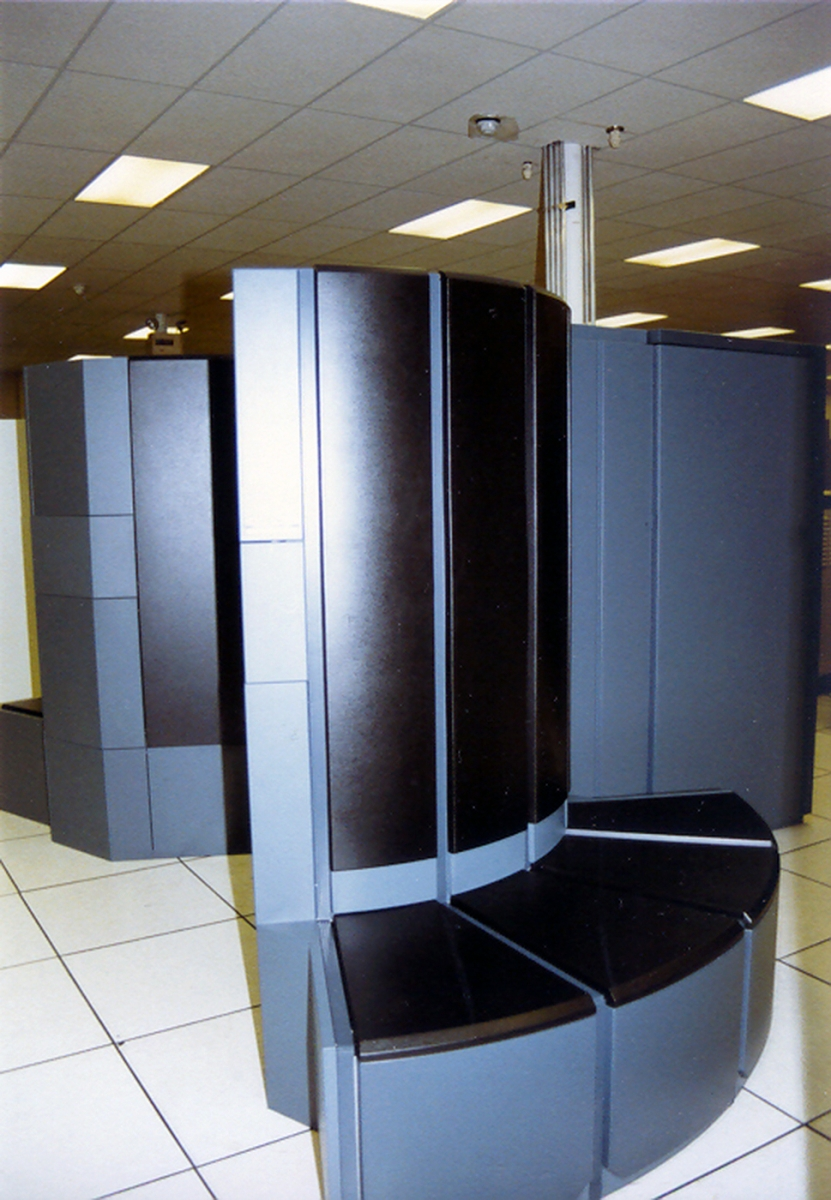
\includegraphics[scale=0.1]{./Cray_Y-MPb.jpg}
  \caption{Ohio State Cray Y-MP supercomputer, ca. 1989.  World's
    fastest computer at the time.  333 MFlop top speed, 512 Mb RAM.}
\end{figure}

\item[1990's:] ``Chemical accuracy'' era---very precise solutions routinely
available, for a cost!  See
\href{http://www.crc.nd.edu/~wschnei1/courses/CBE_547/Resources/1994_WFS_JPC.pdf}{Schneider,
{\em J. Phys. Chem.}, 1994}.

\item[1990's:] Density functional theory (DFT) allows applications to
  solids/surfaces/liquids to become common. See
\href{http://www.crc.nd.edu/~wschnei1/courses/CBE_547/Resources/1998_Hass_Science.pdf}{Hass,
  {\em Science}, 1998}

\item[1990's:] Visualization moves to the desktop

\item[2000's:] Computational ``screening'', materials ``discovery''
See \href{http://www.crc.nd.edu/~wschnei1/courses/CBE_547/Resources/2009_Greeley_JPCc.pdf}{Greeley,
{\em J. Phys. Chem. C}, 2009}.  Also see
\href{http://www.crc.nd.edu/~wschnei1/courses/CBE_547/Resources/2010_Gurkan_JPCL.pdf}{Gurkan,
{\em J. Phys. Chem. Lett.}, 2010}.

\item[Today:] Computational ``chemistry'' widely integrated into all aspects
of chemical, materials, biological research
\end{description}

\subsection{Our goals}
``Computational chemistry'' is now so vast it is impossible to cover
everything completely.  We limit ourselves to quantum-mechanics-based
calculations.

\begin{enumerate}
\item Understand when it is appropriate to use quantum-mechanics
  methods.
\item Be able to state the basic theoretical, mathematical, and numerical
  concepts behind quantum mechanical “wavefunction theory” (WFT) and
  “density functional theory,” (DFT) calculations.  
\item Understand the terminology and practical issues associated with doing quantum chemical simulations.
\item Get hands-on experience with these concepts using popular
  computational tools of today, including GAMESS for molecular
  systems and Vasp for condensed phase systems.
\item Learn how to apply the results of quantum chemical
  simulations to calculate
  things you care about.
\item Demonstrate an ability to formulate a problem and apply QM
  methods to it.
\item Develop the skills to understand a literature paper in the area.
\end{enumerate}
\end{document}

